\documentclass{beamer}

\usetheme{CambridgeUS}
\usecolortheme{orchid}

\usepackage[utf8]{inputenc}
\usepackage[T1]{fontenc}

% Paths
\newcommand{\figs}{../figs}
\newcommand{\data}{../data}
\newcommand{\code}{../code}

% URL styles
\usepackage{url}
\urlstyle{sf}

% Units
\usepackage[detect-weight=true, binary-units=true]{siunitx}
\DeclareSIUnit\flop{Flops}

% Math
\usepackage{amsmath}
\usepackage{amssymb}
\usepackage{bm}
\usepackage{nicefrac}
\newcommand{\dif}[1]{{\;\text{d}#1}}

% Graphics
\usepackage{graphicx}
\usepackage{caption}
\usepackage{subcaption}
\graphicspath{{../figs/}}

% Tikz
\usepackage{tikz}
\usetikzlibrary{positioning,shapes,arrows,calc,intersections}
\usepackage{pgfplots}
\usepgfplotslibrary{dateplot}
\pgfplotsset{compat=1.8}

% Colors
\definecolor{darkblue}{HTML}{00688B}
\definecolor{darkgreen}{HTML}{6E8B3D}
\definecolor{cadet}{HTML}{DAE1FF}
\definecolor{salmon}{HTML}{FFB08A}

% Listings
\usepackage{textcomp}
\usepackage{listings}
\lstset{
  keywordstyle=\bfseries\color{orange},
  stringstyle=\color{darkblue!80},
  commentstyle=\color{darkblue!80},
  showstringspaces=false,
  basicstyle=\ttfamily,
  upquote=true,
}
\lstdefinestyle{fortran}{
  language=Fortran,
  morekeywords={for},
  deletekeywords={status},
}
\lstdefinestyle{c}{
  language=C,
  morekeywords={include},
}
\lstdefinestyle{glsl}{
  language=C,
  morekeywords={attribute, vec2, vec3, vec4, varying, uniform, mat2, mat3, mat4},
}
\lstdefinestyle{cuda}{
  language=C,
  morekeywords={__global__, __device__, __host__},
}
\lstdefinestyle{shell}{
  language=bash,
  morekeywords={mkdir, ssh, cmake},
}

% Double hlines
\usepackage{hhline}

% Misc
\usepackage{nth}

\subtitle{TMA4280---Introduction to Supercomputing}

\begin{document}


\title{The Poisson problem}
\author{Eivind Fonn}
\institute{SINTEF ICT / NTNU}
\date{December 2015}
\maketitle

\begin{frame}
  \frametitle{The Poisson problem}
  \begin{itemize}
  \item The Poisson equation is an elliptic partial differential equation.
  \item The Poisson \emph{problem} is the solution of the Poisson
    \emph{equation} equipped with a set of boundary conditions.
  \item The equation is
    \[
      -\nabla^2 u = f, \qquad \text{ in } \Omega
    \]
    where $u$ is the unknown, $f$ is the load on the system and $\Omega$ denotes
    some domain.
  \item We remark that $\nabla^2$ is the sum of the second order partial
    derivatives, e.g. in one and two dimensions the equation is
    \[
      -u_{xx} = f, \qquad -\left( u_{xx} + u_{yy} \right) = f.
    \]
  \end{itemize}
\end{frame}

\begin{frame}[fragile]
  \frametitle{The Poisson problem}
  \begin{itemize}
  \item This problem is important because a number of physical processes are
    modelled either entirely or in part by the Poisson equation.
  \item The technical term is a \emph{diffusion process}: $u$ is to be
    interpreted as the concentration of ``something'', and $f$ as the rate at
    which ``something'' is introduced ($f > 0$) or removed ($f < 0$) from the
    domain.
  \item ``Something'' may be particles, but also abstract notions such as heat
    or potentials.
  \item The solution in $\Omega$ is uniquely determined by the boundary data and
    $f$.
  \end{itemize}
\end{frame}

\begin{frame}[fragile]
  \frametitle{Electrostatics}
  \begin{itemize}
  \item The differential forms for the electric field $\bm E$ are
    \[
      \begin{split}
        \nabla \cdot \bm E &= 4\pi\rho \\
        \nabla \times \bm E &= 0,
      \end{split}
    \]
    where $\rho$ is the charge density.
  \item The electric field $\bm E$ can be expressed as the gradient of
    a scalar potential $\varphi$, i.e. $\bm E = -\nabla\varphi$. Thus
    \[
      \nabla \cdot \bm E = -\nabla\cdot\nabla\varphi = -\nabla^2\varphi = 4\pi\rho.
    \]
  \end{itemize}
\end{frame}

\begin{frame}
  \frametitle{Potential flow}
  \begin{itemize}
  \item Likewise, potential flow in fluid mechanics can be modelled by this
    equation.
  \item Given a velocity field $\bm U$ which is irrotational and incompressible,
    \[
      \begin{split}
        \nabla \times \bm U &= 0 \\
        \nabla \cdot \bm U &= 0,
      \end{split}
    \]
    it follows that $\bm U = \nabla\varphi$ where $\varphi$ is a scalar velocity
    potential, which satisfies the Laplace equation
    \[
      \nabla^2\varphi = 0.
    \]
  \end{itemize}
\end{frame}

\begin{frame}[fragile]
  \frametitle{Steady heat transfer}
  Energy transfered out of an arbitrary domain $V$ can be expressed as
  \[
    \int_{\partial V} \bm q \cdot \bm n \dif{S} = \int_V f \dif{V}.
  \]
  where $\bm q$ is the heat flux, $\bm n$ is the outward surface normal along
  the boundary $\partial V$ and $f$ represents a volumetric heat source. This
  basically says that the net energy generation inside the domain must equal the
  net energy flowing out of the domain.
  \begin{center}
    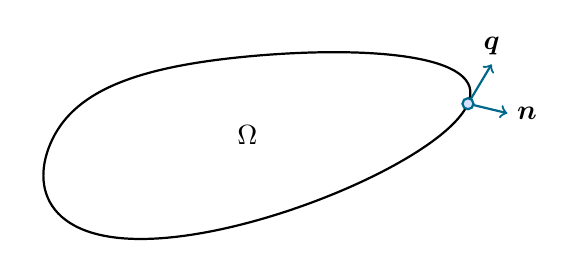
\begin{tikzpicture}
  \draw[thick] plot [smooth cycle, tension=1.0] coordinates {
    (0,-0.1) (1.5,-1.3) (5.3,0.4) (2.5,1)};
  \node at (2.5,0) {$\Omega$};
  \draw[darkblue, thick, ->] (5.3,0.4) -- (5.8,0.28);
  \node[anchor=west] at (5.8,0.28) {$\bm n$};
  \draw[darkblue, thick, ->] (5.3,0.4) -- (5.6,0.9);
  \node[anchor=south] at (5.6,0.9) {$\bm q$};
  \draw[darkblue, fill=cadet, thick] (5.3,0.4) circle (0.07);
\end{tikzpicture}

  \end{center}
\end{frame}

\begin{frame}[fragile]
  \frametitle{Steady heat transfer}
  \begin{itemize}
  \item Applying the Gauss' divergence theorem, we can write
    \[
      \int_{\partial V} \bm q \cdot \bm n \dif{S}
      = \int_V \nabla \cdot \bm q \dif{V}
      = \int_V f \dif{V},
    \]
    yielding
    \[
      \nabla \cdot \bm q = f.
    \]
  \item Applying Fourier's law, i.e. $\bm q = -\kappa \nabla u$, $\kappa > 0$,
    we get
    \[
      - \nabla\cdot\kappa\nabla u = f \qquad \text{ in } \Omega,
    \]
    to be solved for the temperature $u$.
  \item For a constant isotropic heat conductivity $\kappa$, we regain the
    Poisson equation,
    \[
      - \kappa\nabla^2 u = f.
    \]
  \end{itemize}
\end{frame}

\begin{frame}
  \frametitle{Unsteady heat transfer}
  \begin{itemize}
  \item Unsteady heat transfer is modelled by the heat equation
    \[
      \frac{\partial u}{\partial t} = \kappa\nabla^2u + f \qquad \text{ in } \Omega.
    \]
  \item Discretizing in time using Backward Euler, we otain
    \[
      \frac{1}{\Delta t} (u^{n+1}-u^n) = \kappa\nabla^2u^{n+1}+f^{n+1}
    \]
    where superscript $n$ refers to a quanity at time $t^n, n=0,1,\ldots$.
  \item This can be written as
    \[
      \left(-\kappa\nabla^2 + \frac{1}{\Delta t}\right)u^{n+1} = \frac{u^n}{\Delta t}+f^{n+1}.
    \]
  \item This is a \emph{Helmholtz} equation: Laplacian plus a multiple of the
    identity.
  \end{itemize}
\end{frame}

\begin{frame}[fragile]
  \frametitle{Solving PDEs on computers}
  \begin{itemize}
  \item Typically we can only solve the equation in an approximate sense.
  \item Computers can only work on finite-dimensional data.
  \item The process of approximating a continuous equation with a finite
    dimensional one is called \emph{discretizing} the equation.
  \item Several ways to do this.
  \item The most popular ones:
    \begin{itemize}
    \item finite differences,
    \item finite volumes,
    \item finite elements.
    \end{itemize}
  \end{itemize}
\end{frame}

\begin{frame}[fragile]
  \frametitle{Solving PDEs on computers}
  \begin{itemize}
  \item This is not a course in discretization of PDEs.
  \item We will concentrate on the finite difference approach since it is the
    least technical.
  \item However, all of them have something in common: At the end of the day you
    end up with a set of linear equations to solve,
    \[
      \bm A \bm u = \bm g
    \]
    where $\bm A$ is the matrix of linear equations, $\bm u$ the unknown
    solution and $\bm g$ the discretized load on the system (the right hand
    side).
  \item We will focus mostly on solving the equations, and thus most of what we
    consider is applicable no matter the discretization approach.
  \end{itemize}
\end{frame}

\begin{frame}
  \frametitle{Finite difference methods}
  \begin{itemize}
    \item Consider a continuous function 1D function $u(x)$.
    \item Introduce a grid, $\left\{x_i\right\}_{i=0}^N$, with $x_i = x_0+ih$.
    \item Here $h$ is the grid spacing. For simplicity we consider equidistant
      grids (constant $h$).
      \begin{center}
        \scalebox{0.7}{\begin{tikzpicture}
  \begin{axis}[
    xmin=-1,
    xmax=1,
    ymin=0,
    ymax=6,
    axis lines=middle,
    axis x line=center,
    hide y axis,
    xtick={-0.7,0.001,0.7},
    xticklabels={$x_i-h$,$x_i$,$x_i+h$},
    xlabel={$x$},
    ]
    \addplot[darkblue, thick, domain=-1:1, samples=100]{x^3+3};
    \draw[thin, densely dashed] (axis cs:0.001,0) -- (axis cs:0,3);
    \draw[thin, densely dashed] (axis cs:-0.7,0) -- (axis cs:-0.7,2.657);
    \draw[thin, densely dashed] (axis cs:0.7,0) -- (axis cs:0.7,3.343);
    \node[shape=circle, draw=darkblue, thick, fill=cadet, inner sep=0.5mm] at (axis cs:-0.7,2.657) {};
    \node[shape=circle, draw=darkblue, thick, fill=cadet, inner sep=0.5mm] at (axis cs:0,3) {};
    \node[shape=circle, draw=darkblue, thick, fill=cadet, inner sep=0.5mm] at (axis cs:0.7,3.343) {};
    \node[anchor=east, xshift=-3mm] at (axis cs:1,4) {$u(x)$};
  \end{axis}
\end{tikzpicture}
}
      \end{center}
    \item Want to approximate derivatives of the function only using data on the grid.
  \end{itemize}
\end{frame}

\begin{frame}
  \frametitle{Finite differences}
  \begin{itemize}
  \item First idea: How derivatives were introduced in high school:
    \[
      u'(x_i) \approx \frac{1}{h} \left( u(x_i+h)-u(x_i) \right).
    \]
  \item This is called a one-sided difference (a \emph{forward} difference).
    Invoking Taylor we find
    \begin{align*}
      \frac{1}{h} \left( u(x_i+h)-u(x_i) \right)
      &= \frac{1}{h} \left( u(x_i) + hu'(x_i) + \mathcal{O}(h^2) - u(x_i) \right) \\
      &= u'(x_i) + \mathcal{O}(h)
    \end{align*}
    In other words, this is a \emph{first order} approximation to $u'(x_i)$.
  \end{itemize}
\end{frame}

\begin{frame}
  \frametitle{Finite differences}
  \begin{itemize}
  \item Second idea: a centered difference
    \[
      u'(x_i) \approx \frac{1}{2h} \left( u(x_i + h) - u(x_i - h) \right).
    \]
  \item Invoking Taylor we find
    \[
      \frac{1}{2h} \left( u(x_i + h) - u(x_i - h) \right)
      = u'(x_i) + \mathcal{O}(h^2).
    \]
    In other words, this is a \emph{second order} approximation to $u'(x_i)$.
  \end{itemize}
\end{frame}

\begin{frame}
  \frametitle{Finite difference methods}
  \begin{itemize}
  \item A centered difference for the second derivative:
    \begin{align*}
      u''(x_i) &\approx \frac{1}{h}\left( u'(x_i + \nicefrac{h}{2}) - u'(x_i - \nicefrac{h}{2})\right) \\
      &\approx \frac{1}{h^2}\left( u(x_i + h) - 2u(x_i) + u(x_i - h) \right)
    \end{align*}
  \item Invoking Taylor we find
    \[
      \frac{1}{h^2}\left( u(x_i + h) - 2u(x_i) + u(x_i - h) \right)
      = u''(x_i) + \mathcal{O}(h^2).
    \]
    In other words, this is a \emph{second order} approximation to $u''(x_i)$.
  \end{itemize}
\end{frame}

\begin{frame}
  \frametitle{Stencils}
  Finite differences are often illustrated using \emph{stencils}.
  \begin{figure}
    \begin{center}
      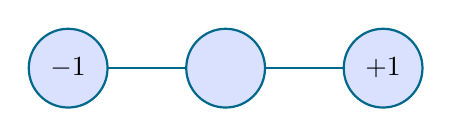
\begin{tikzpicture}[
  every node/.style={
    shape=circle,
    thick,
    fill=cadet,
    draw=darkblue,
    minimum size=1cm,
  }]
  \draw[thick, darkblue] (-2,0) -- (2,0);
  \node at (-2,0) {$-1$};
  \node at (0,0) {};
  \node at (2,0) {$+1$};
\end{tikzpicture}

    \end{center}
    \caption{Stencil for the first derivative (central difference)}
  \end{figure}
  \begin{figure}
    \begin{center}
      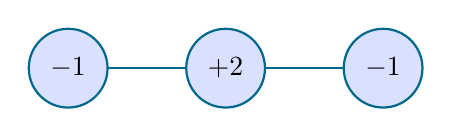
\begin{tikzpicture}[
  every node/.style={
    shape=circle,
    thick,
    fill=cadet,
    draw=darkblue,
    minimum size=1cm,
  }]
  \draw[thick, darkblue] (-2,0) -- (2,0);
  \node at (-2,0) {$-1$};
  \node at (0,0) {$+2$};
  \node at (2,0) {$-1$};
\end{tikzpicture}

    \end{center}
    \caption{Stencil for the second derivative}
  \end{figure}
\end{frame}

\begin{frame}[fragile]
  \frametitle{Discretization in 1D}
  \begin{itemize}
  \item We now consider the 1D Poisson problem
    \[
      \begin{split}
        -u_{xx} &= f, \qquad \text{ in } \Omega = (0,1), \\
        u(0) &= u(1) = 0.
      \end{split}
    \]
    \begin{center}
      \scalebox{0.7}{\begin{tikzpicture}
  \begin{axis}[
    xmin=-10,
    xmax=190,
    ymin=0,
    ymax=3,
    axis lines=middle,
    axis x line=center,
    hide y axis,
    xtick={1,180},
    xticklabels={$x=0$, $x=1$},
    ]
    \addplot[darkblue, thick, domain=0:180, samples=100]{sin(x) - 0.4*sin(2*x)};
    \node[anchor=west] at (axis cs:140,1.2) {$u(x)$};
  \end{axis}
\end{tikzpicture}
}
    \end{center}
  \item These are called homogenous Dirichlet boundary conditions: the solution
    is prescribed to be zero on the boundaries of the domain.
  \item Introduce the grid, $\left\{x_i\right\}_{i=0}^N$, with $x_i = x_0+ih$,
    $h = \nicefrac{1}{N}$.
    \begin{center}
      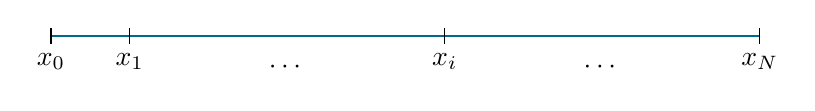
\begin{tikzpicture}
  \draw[thick, darkblue] (0,0) -- (9,0);
  \foreach \i in {0, 1, 5, 9} {
    \draw[thin] (\i,-0.1) -- (\i,0.1);
  }
  \node[anchor=north] at (0,-0.1) {$x_0$};
  \node[anchor=north] at (1,-0.1) {$x_1$};
  \node[anchor=north] at (3,-0.2) {$\cdots$};
  \node[anchor=north] at (5,-0.1) {$x_i$};
  \node[anchor=north] at (7,-0.2) {$\cdots$};
  \node[anchor=north] at (9,-0.1) {$x_N$};
\end{tikzpicture}

    \end{center}
  \end{itemize}
\end{frame}

\begin{frame}
  \frametitle{Discretization in 1D}
  \begin{itemize}
  \item Let $u_i$ denote $u(x_i)$ and $f_i$ denote $f(x_i)$.
  \item Due to the boundary conditions we know that $u_0 = u_N = 0$.
  \item We thus have $N-1$ unknowns. We collect these in a vector $\bm u$.
  \item We then apply the second order finite difference formula in each grid
    point.
    \begin{align*}
      - \frac{1}{h^2} \left(u_{i+1} - 2u_i + u_{i-1} \right) &= f_i, \qquad i=1,\ldots,n-1, \\
      u_0 &= u_N = 0.
    \end{align*}
  \end{itemize}
\end{frame}

\begin{frame}
  \frametitle{Discretization in 1D}
  These equations can also be expressed as the system
  \begin{align*}
    2u_1 - u_2 &= h^2 f_2 \\
    -u_1 + 2u_2 - u_3 &= h^2 f_3 \\
               &\vdots \\
    -u_{N-2} + 2u_{N-1} &= h^2 f_{N-1},
  \end{align*}
  or in matrix form
  \begin{align*}
    \underbrace{ \begin{pmatrix}
      2 & -1 & & & \\
      -1 & 2 & -1 & & \\
      & & \ddots & & \\
      & & -1 & 2 & -1 \\
      & & & -1 & 2
    \end{pmatrix}
    }_{\bm A}
    \underbrace{ \begin{pmatrix}
      u_1 \\
      u_2 \\
      \vdots \\
      u_{n-2} \\
      u_{n-1}
    \end{pmatrix}
    }_{\bm u}
    &= h^2
    \underbrace{ \begin{pmatrix}
      f_1 \\
      f_2 \\
      \vdots \\
      f_{n-2} \\
      f_{n-1}
    \end{pmatrix}
    }_{\bm f} ,
  \end{align*}
\end{frame}

\begin{frame}
  \frametitle{Discretization in 1D}
  \begin{itemize}
  \item The matrix $\bm A$ is sparse (tridiagonal).
  \item The matrix $\bm A$ is symmetric, that is $\bm A = \bm A^\intercal$.
  \item The matrix $\bm A$ is positive definite, that is,
    $\bm v^\intercal \bm A \bm v > 0$
    for all vectors $\bm v \in \mathbb{R}^{N-1}$, $\bm v \not= \bm 0$.
  \item Thus, the system of $N-1$ equations is solvable and has a unique
    solution.
  \item The error in the grid points is of second order, i.e.
    $|u(x_i)-u_i| \sim \mathcal{O}(h^2)$.
  \end{itemize}
\end{frame}

\begin{frame}
  \frametitle{Discretization in 2D}
  If the domain $\Omega$ is rectangular, we can use two independent grids
  $\{x_i\}_{i=0}^N$ and $\{y_j\}_{j=0}^M$in the $x$ and $y$-directions.
  \begin{center}
    \scalebox{0.7}{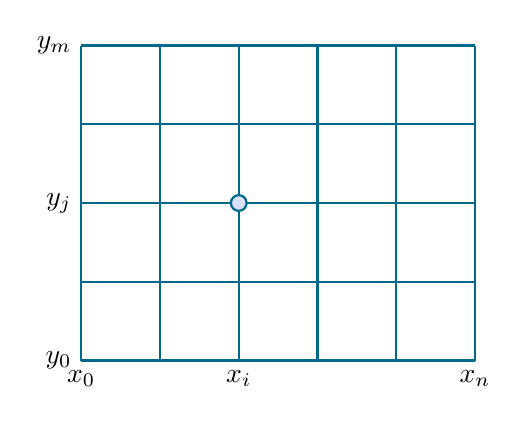
\begin{tikzpicture}[scale=0.5]
  \foreach \i in {0,2,4,6,8,10} {
    \draw[thick, darkblue] (\i,0) -- (\i,8);
  }
  \foreach \j in {0,2,4,6,8} {
    \draw[thick, darkblue] (0,\j) -- (10,\j);
  }
  \draw[thick, darkblue, fill=cadet] (4,4) circle (2mm);
  \node[anchor=east] at (0,0) {$y_0$};
  \node[anchor=east] at (0,4) {$y_j$};
  \node[anchor=east] at (0,8) {$y_m$};
  \node[anchor=north] at (0,0) {$x_0$};
  \node[anchor=north] at (4,0) {$x_i$};
  \node[anchor=north] at (10,0) {$x_n$};
\end{tikzpicture}
}
  \end{center}
  \begin{align*}
    x_i &= x_0 + ih_x, \\
    y_j &= y_0 + jh_y.
  \end{align*}
\end{frame}

\begin{frame}
  \frametitle{Finite differences in 2D}
  We need to approximate $u_{xx} + u_{yy}$ at a point $(x_i, y_j)$. Therefore,
  we use two one-dimensional finite differences,
  \begin{align*}
    u_{xx}(x_i, y_i) &\approx \frac{1}{h_x^2}
                       \left( u_{i-1,j} - 2u_{i,j} + u_{i+1,j} \right) \\
    u_{yy}(x_i, y_i) &\approx \frac{1}{h_y^2}
                       \left( u_{i,j-1} - 2u_{i,j} + u_{i,j+1} \right) \\
  \end{align*}
  If $h_x = h_y = h$ we get
  \[
    \nabla u(x_i, y_i) \approx \frac{1}{h^2}
    \left( u_{i-1,j} + u_{i+1,j} + u_{i,j-1} + u_{i,j+1} - 4u_{i,j} \right)
  \]
\end{frame}

\begin{frame}
  \frametitle{Finite differences in 2D}
  This is known as the \emph{five-point} stencil. (The signs are flipped because
  the Poisson equation involves $-\nabla$.)
  \begin{center}
    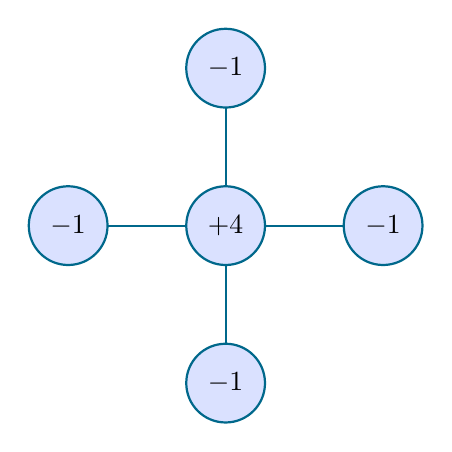
\begin{tikzpicture}[
  every node/.style={
    shape=circle,
    thick,
    fill=cadet,
    draw=darkblue,
    minimum size=1cm,
  }]
  \draw[thick, darkblue] (-2,0) -- (2,0);
  \draw[thick, darkblue] (0,-2) -- (0,2);
  \node at (-2,0) {$-1$};
  \node at (2,0) {$-1$};
  \node at (0,-2) {$-1$};
  \node at (0,2) {$-1$};
  \node at (0,0) {$+4$};
\end{tikzpicture}

  \end{center}
\end{frame}

\begin{frame}
  \frametitle{Node numbering in 2D}
  Numbering nodes is not as trivial in 2D as in 1D. We use a ``natural''
  ordering of the unknowns: we first number all the \emph{internal} nodes along
  ``row'' 1 (in the $x$-direction), followed by the nodes in ``row'' 2, etc.
  \begin{center}
    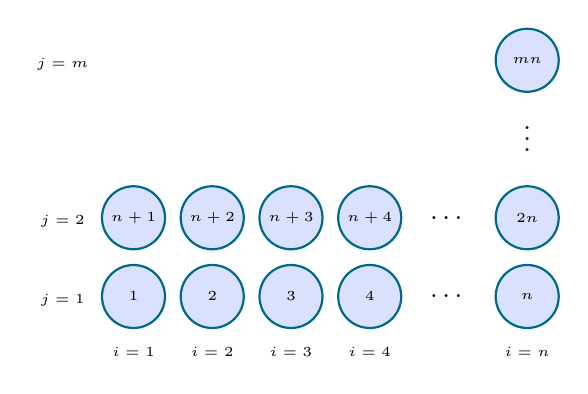
\begin{tikzpicture}[
  block/.style={
    shape=circle,
    thick,
    draw=darkblue,
    fill=cadet,
    inner sep=0.2mm,
    minimum size=8mm,
  }]
  \node[block] at (0,0) {\tiny $1$};
  \node[block] at (1,0) {\tiny $2$};
  \node[block] at (2,0) {\tiny $3$};
  \node[block] at (3,0) {\tiny $4$};
  \node at (4,0) {\ldots};
  \node[block] at (5,0) {\tiny $n$};

  \node[block] at (0,1) {\tiny $n+1$};
  \node[block] at (1,1) {\tiny $n+2$};
  \node[block] at (2,1) {\tiny $n+3$};
  \node[block] at (3,1) {\tiny $n+4$};
  \node at (4,1) {\ldots};
  \node[block] at (5,1) {\tiny $2n$};

  \node[yshift=1mm] at (5,2) {$\vdots$};
  \node[block] at (5,3) {\tiny $mn$};

  \node at (0,-0.7) {\tiny $i=1$};
  \node at (1,-0.7) {\tiny $i=2$};
  \node at (2,-0.7) {\tiny $i=3$};
  \node at (3,-0.7) {\tiny $i=4$};
  \node at (5,-0.7) {\tiny $i=n$};
  \node at (-0.9,-0.05) {\tiny $j=1$};
  \node at (-0.9,0.95) {\tiny $j=2$};
  \node at (-0.9,2.95) {\tiny $j=m$};
\end{tikzpicture}

  \end{center}
\end{frame}

\begin{frame}
  \frametitle{Matrix block structure}
  The final linear system will have a block-like structure,
  \[
    \underbrace{
      \begin{pmatrix}
        \bm A_0 & \bm A_1 & & & \\
        \bm A_1 & \bm A_0 & \bm A_1 & & \\
        & \bm A_1 & \bm A_0 & \ddots & \\
        & & \ddots & \ddots & \bm A_1 \\
        & & & \bm A_1 & \bm A_0
      \end{pmatrix}}_{\bm A}
    \underbrace{
      \begin{pmatrix}
        u_1 \\ u_2 \\ u_3 \\ \vdots \\ u_N
      \end{pmatrix}}_{\bm u}
    =
    \underbrace{
      \begin{pmatrix}
        f_1 \\ f_2 \\ f_3 \\ \vdots \\ f_N
      \end{pmatrix}}_{\bm g}
  \]
\end{frame}

\begin{frame}
  \frametitle{Matrix block structure}
  The blocks $\bm A_0$ and $\bm A_1$ can be written as
  \[
    \bm A_0 =
    \begin{pmatrix}
      4 & -1 & & & \\
      -1 & 4 & -1 & & \\
      & -1 & 4 & \ddots & \\
      & & \ddots & \ddots & -1 \\
      & & & -1 & 4
    \end{pmatrix}
    \qquad
    \bm A_1 =
    \begin{pmatrix}
      -1 & & & & \\
      & -1 & & & \\
      & & -1 & & \\
      & & & \ddots & \\
      & & & & -1
    \end{pmatrix}.
  \]
\end{frame}

\end{document}

